%% bare_jrnl.tex
%% V1.4b (2015/08/26) by Michael Shell
%% Modified for: ACDCB manuscript submission

\documentclass[journal]{IEEEtran}

% *** MATH PACKAGES ***
\usepackage{amsmath}
\usepackage{amssymb}
\usepackage{amsfonts}
\interdisplaylinepenalty=2500

% *** CITATION PACKAGES ***
\usepackage{cite}

% *** GRAPHICS RELATED PACKAGES ***
\ifCLASSINFOpdf
  \usepackage[pdftex]{graphicx}
  \graphicspath{{../figures/presentation_highres/}}
  \DeclareGraphicsExtensions{.pdf,.png}
\else
  \usepackage[dvips]{graphicx}
  \graphicspath{{../figures/presentation_highres/}}
  \DeclareGraphicsExtensions{.eps}
\fi

% *** ALIGNMENT PACKAGES ***
\usepackage{array}
\usepackage{booktabs}

% *** FLOAT PACKAGES ***
\usepackage{stfloats}

% *** PDF, URL AND HYPERLINK PACKAGES ***
\usepackage{url}

% correct bad hyphenation here
\hyphenation{op-tical net-works semi-conduc-tor XGBoost Light-GBM}

\begin{document}

% --- Title ---
\title{ACDCB: Age-Conditioned Dual-Space Constrained Blending for Concrete Compressive Strength Prediction}

% --- Authors ---
\author{Author~Names,~\IEEEmembership{Institution,~City,~Country}
\thanks{Manuscript received xxx; revised xxx.}}

\markboth{IEEE Transactions on Engineering Structures,~Vol.~XX, No.~X, Month~2026}%
{Author \MakeLowercase{\textit{et al.}}: ACDCB for Concrete Strength Prediction}

\maketitle

% --- Abstract ---
\begin{abstract}
This study proposes ACDCB (Age-Conditioned Dual-Space Constrained Blending), a novel ensemble learning framework designed to predict the compressive strength of concrete by capturing complex, age-dependent nonlinear mappings. The framework integrates dual feature spaces---a 32-dimensional primary space and a 22-dimensional anchor space---to balance expressiveness and robustness. Using four gradient-boosted tree models (XGBoost, LightGBM, and HistGradientBoosting), ACDCB employs a constrained weight optimization (SLSQP) strategy. To reflect concrete maturity physics, the blending weights are optimized separately for early-age ($\leq 28$ days) and late-age ($>28$ days) regimes. Validated on the UCI dataset, ACDCB achieved an $R^2$ of 0.9488 and an RMSE of 3.70\,MPa, marking a 25.6\% reduction in RMSE over the AdaBoost baseline. Ablation experiments demonstrate that the anchor space is critical for stability, while the piecewise blending provides physical interpretability: the anchor model dominates early-age predictions, whereas XGBoost's importance grows in late-age regimes. ACDCB offers a principled, modular, and physics-aware approach to material strength modeling, providing a significant improvement in both predictive accuracy and model interpretability for structural engineering applications.
\end{abstract}

\begin{IEEEkeywords}
concrete compressive strength, ensemble learning, age-conditioned blending, constrained optimization, dual feature spaces, gradient boosting.
\end{IEEEkeywords}

\IEEEpeerreviewmaketitle

%==========================================================================
\section{Introduction}
%==========================================================================

\IEEEPARstart{T}{he} accurate prediction of concrete compressive strength is a cornerstone problem in structural engineering, with direct implications for construction scheduling, quality control, and service-life assessment \cite{yeh1998concrete}. Traditional approaches rely on empirical regression formulas---such as Abrams' law or power-law maturity models---that offer computational simplicity but cannot adequately capture the high-dimensional, nonlinear interactions among mix design variables, admixture effects, and curing conditions \cite{yeh2006analysis}.

Over the past two decades, machine learning (ML) methods have emerged as powerful alternatives. Artificial neural networks (ANN), support vector machines (SVM), and ensemble methods---particularly AdaBoost with decision tree weak learners---have demonstrated progressively improving predictive accuracy on the UCI benchmark dataset \cite{yeh1998concrete,chou2014machine}. Notably, the AdaBoost-based approach reported by Feng et al.\ \cite{feng2020machine} achieved a 10-fold cross-validated $R^2$ of approximately 0.95 and RMSE below 5\,MPa, establishing a strong baseline for subsequent work.

However, three structural limitations persist across existing approaches:

\begin{enumerate}
\item \textbf{Mono-representation}: All models operate on a single feature space---typically the raw mix proportions or a fixed set of engineered ratios. No existing framework systematically exploits \emph{complementary} feature representations that trade off expressiveness and robustness.

\item \textbf{Age-agnostic integration}: While concrete strength development is fundamentally age-dependent---governed by distinct hydration kinetics in early ($\leq 28$ days) versus later ages---most ensemble methods apply uniform blending weights across all ages, failing to adapt to regime-specific model competencies.

\item \textbf{Unconstrained model combination}: Standard ensemble stacking and averaging impose no formal constraints on combination weights. Negative or unbounded weights, while occasionally improving point estimates, obscure interpretability and can produce physically implausible extrapolations.
\end{enumerate}

To address these gaps, we propose \textbf{ACDCB} (Age-Conditioned Dual-Space Constrained Blending), a framework characterized by four design principles:

\begin{itemize}
\item \textbf{Dual Feature Spaces (D)}: Two feature representations---\emph{primary} (32 dimensions, expression-oriented) and \emph{anchor} (22 dimensions, robustness-oriented)---are constructed from the same 8 base variables through systematic civil engineering feature engineering. Each space feeds a dedicated subset of base models.

\item \textbf{Constrained Blending (C, B)}: Model combination weights are learned through constrained optimization (SLSQP), minimizing RMSE subject to the convex constraints $w_i \geq 0$ and $\sum_i w_i = 1$. This ensures weights are directly interpretable as ``contribution shares.''

\item \textbf{Age Conditioning (A, C)}: The dataset is partitioned at the 28-day curing threshold---a physically meaningful engineering landmark---and separate blending weights are optimized for each regime.

\item \textbf{Multi-Model Pool}: Four gradient-boosted tree variants (XGBoost, LightGBM, HistGradientBoosting, and an anchor-space HistGradientBoosting) constitute the candidate model pool, selected for their complementary inductive biases.
\end{itemize}

The remainder of this paper is organized as follows. Section~2 describes the experimental database and preprocessing pipeline. Section~3 presents the mathematical foundations of the baseline models and the ACDCB framework. Section~4 details the implementation and training strategy. Section~5 reports model validation and evaluation results. Section~6 presents the ablation study decomposing component contributions. Section~7 provides comparative analysis against prior work. Sections~8 and~9 offer discussion and conclusions, respectively.

%==========================================================================
\section{Experimental Database}
%==========================================================================

\subsection{Data Source}

This study employs the UCI Concrete Compressive Strength dataset \cite{yeh1998concrete}, publicly available from the UCI Machine Learning Repository (DOI: 10.24432/C5PK67). The dataset comprises 1{,}030 experimental observations, each characterized by 8 input variables describing concrete mix proportions and curing age, along with one output variable---the 28-day (or specified-age) compressive strength in MPa.

\subsection{Input Variables}

The eight base features, their physical interpretations, and measurement units are summarized in Table~\ref{tab:variables}.

\begin{table}[!t]
\renewcommand{\arraystretch}{1.2}
\caption{Input Variables for Concrete Compressive Strength Prediction}
\label{tab:variables}
\centering
\begin{tabular}{ccp{4.2cm}c}
\toprule
\textbf{Variable} & \textbf{Symbol} & \textbf{Description} & \textbf{Unit} \\
\midrule
Cement            & $C$    & Portland cement content              & kg/m$^3$ \\
Blast Furnace Slag& $S$    & Ground granulated blast-furnace slag & kg/m$^3$ \\
Fly Ash           & $FA$   & Class F/C fly ash                    & kg/m$^3$ \\
Water             & $W$    & Mixing water                         & kg/m$^3$ \\
Superplasticizer  & $SP$   & High-range water-reducing admixture  & kg/m$^3$ \\
Coarse Aggregate  & $CA$   & Coarse aggregate ($>$4.75\,mm)       & kg/m$^3$ \\
Fine Aggregate    & $FA_g$ & Fine aggregate ($<$4.75\,mm)         & kg/m$^3$ \\
Age               & $t$    & Curing age                           & days \\
\bottomrule
\end{tabular}
\end{table}

\textbf{Target variable}: $f_c$ --- Concrete compressive strength (MPa).

\subsection{Statistical Summary}

The target variable (compressive strength) exhibits substantial variability: $\mu = 35.82$\,MPa, $\sigma = 16.70$\,MPa, with values spanning 2.33--82.60\,MPa, reflecting diverse mix designs ranging from low-strength to high-performance concrete. The age distribution is heavily right-skewed (skewness $>2.0$), with a concentration of samples at early ages (1--28 days) and a long tail extending to 365 days. This heterogeneous age distribution motivates the age-conditioned design of the ACDCB framework.

Figs.~\ref{fig:corr} and~\ref{fig:violin} present the Pearson correlation heatmap and violin plots of key features, providing a comprehensive view of the data distribution.

\begin{figure}[!t]
\centering
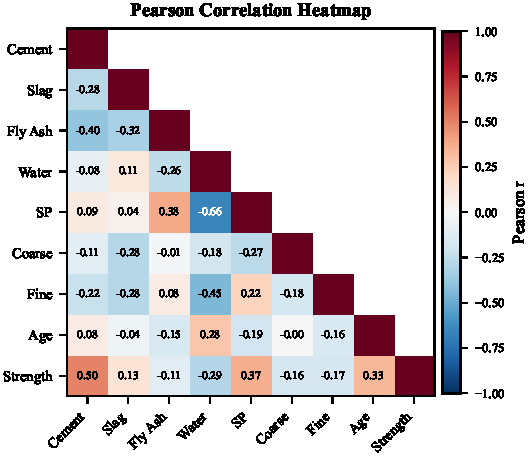
\includegraphics[width=\columnwidth]{fig_corr_heatmap}
\caption{Pearson correlation heatmap of all input variables and the target strength in the UCI dataset.}
\label{fig:corr}
\end{figure}

\begin{figure}[!t]
\centering
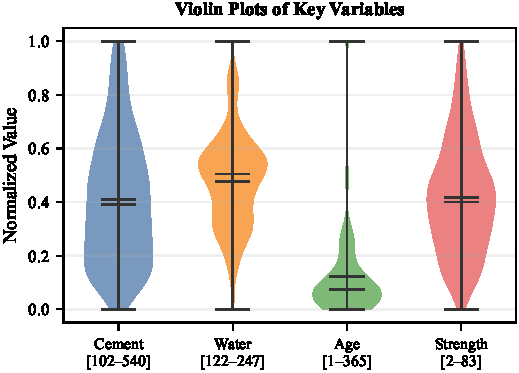
\includegraphics[width=\columnwidth]{fig_violin}
\caption{Violin plots of key features (cement, water, age, strength) showing normalized distributions and value ranges.}
\label{fig:violin}
\end{figure}

\subsection{Feature Engineering}

Beyond the 8 base variables, two tiers of engineered features are constructed to capture known concrete mechanics relationships.

\subsubsection{Tier 1 --- Mechanistic Features}
Shared by primary and anchor spaces, 14 features. Let $\varepsilon = 10^{-6}$ for numerical stability. Define intermediate quantities:
\begin{align}
B &= C + S + FA \quad \text{(total binder)} \label{eq:binder}\\
TA &= CA + FA_g \quad \text{(total aggregate)} \label{eq:agg}\\
t_{\log} &= \log(1 + t) \label{eq:tlog}
\end{align}

The mechanistic features include:
\begin{align}
&\frac{W}{C},\; \frac{W}{B},\; \frac{SP}{B},\; \frac{S + FA}{B},\; \frac{FA_g}{TA} \notag\\
&t_{\log},\; \sqrt{t},\; t^{0.25} \notag\\
&\text{Abrams Index} = \frac{t_{\log}}{W/B},\; C \cdot t_{\log},\; B \cdot t_{\log},\; \frac{W}{B} \cdot t_{\log} \notag\\
&\text{Paste Index} = \frac{C + S + FA + W + SP}{TA} \notag
\end{align}

These features encode well-established concrete engineering principles: water-binder ratio governs ultimate strength (Abrams' law), binder-age interactions capture maturity effects, and paste-to-aggregate ratios reflect volumetric composition.

\subsubsection{Tier 2 --- Enhanced Features}
Primary space only, 10 additional features:
\begin{align}
&\frac{B}{TA},\; \frac{W}{W + B + SP},\; \frac{C}{B},\; \frac{S}{B},\; \frac{FA}{B} \notag\\
&\frac{SP}{W},\; t_{\log} \cdot \frac{B}{W},\; \frac{TA}{B},\; \frac{1}{t + 1},\; t_{\log} \cdot \frac{W}{C} \notag
\end{align}

The primary space thus contains 32 dimensions (8 base $+$ 14 mechanistic $+$ 10 enhanced), while the anchor space contains 22 dimensions (8 base $+$ 14 mechanistic).

After feature engineering, all infinite values (resulting from division by near-zero denominators) are replaced with column medians to maintain data integrity.

%==========================================================================
\section{Methodology}
%==========================================================================

\subsection{Baseline Models}

To establish comparative baselines, we reproduce three representative models from the literature.

\subsubsection{AdaBoost Regression}

AdaBoost (Adaptive Boosting) is an ensemble method that sequentially trains weak learners---here, Classification and Regression Trees (CART)---with adaptive sample weighting \cite{freund1997decision}. For a training set $\mathcal{D} = \{(\mathbf{x}_i, y_i)\}_{i=1}^{m}$, the algorithm proceeds as follows:

\textbf{Step 1 --- Weight initialization}: Each sample receives equal weight $w_{1,i} = 1/m$.

\textbf{Step 2 --- Iterative training}: For iteration $k = 1, \dots, K$:
\begin{enumerate}
\item Train weak learner $G_k(\mathbf{x})$ on the weighted dataset.
\item Compute sample-wise relative error:
\begin{equation}
e_{k,i} = \frac{|y_i - G_k(\mathbf{x}_i)|}{E_k}, \quad E_k = \max_i |y_i - G_k(\mathbf{x}_i)|
\end{equation}
\item Compute the aggregate error and weight coefficient:
\begin{equation}
e_k = \sum_{i=1}^{m} w_{k,i} \cdot e_{k,i}, \quad \alpha_k = \frac{e_k}{1 - e_k}
\end{equation}
\item Update sample weights for the next iteration:
\begin{equation}
w_{k+1,i} = \frac{w_{k,i} \cdot \alpha_k^{1 - e_{k,i}}}{\sum_{j=1}^{m} w_{k,j} \cdot \alpha_k^{1 - e_{k,j}}}
\end{equation}
\end{enumerate}

\textbf{Step 3 --- Ensemble prediction}: The final prediction is the weighted median of all weak learner outputs, with learner weight $\ln(1/\alpha_k)$.

\subsubsection{Artificial Neural Network}

The ANN baseline employs a multi-layer perceptron with one hidden layer of 8 neurons and ReLU activation, following the architecture used in Yeh \cite{yeh1998concrete}:
\begin{align}
\mathbf{h} &= \text{ReLU}(\mathbf{W}^{(1)}\mathbf{x} + \mathbf{b}^{(1)}) \\
\hat{y} &= \mathbf{W}^{(2)}\mathbf{h} + b^{(2)}
\end{align}
where $\mathbf{W}^{(1)} \in \mathbb{R}^{8 \times 8}$, $\mathbf{W}^{(2)} \in \mathbb{R}^{1 \times 8}$. Training minimizes MSE via stochastic gradient descent (SGD) with momentum $\beta = 0.5$:
\begin{equation}
\mathbf{W} \leftarrow \mathbf{W} - \eta \nabla_{\mathbf{W}} \mathcal{L}_{\text{MSE}} + \beta \Delta\mathbf{W}_{\text{prev}}
\end{equation}

\subsubsection{Support Vector Regression}

SVR with radial basis function (RBF) kernel maps inputs to a high-dimensional feature space and fits an $\varepsilon$-insensitive tube:
\begin{equation}
\min_{\mathbf{w}, b, \xi, \xi^*} \frac{1}{2}\|\mathbf{w}\|^2 + C\sum_{i=1}^{m}(\xi_i + \xi_i^*)
\end{equation}
subject to:
\begin{align}
y_i - \mathbf{w}^T\phi(\mathbf{x}_i) - b &\leq \varepsilon + \xi_i \notag\\
\mathbf{w}^T\phi(\mathbf{x}_i) + b - y_i &\leq \varepsilon + \xi_i^* \notag\\
\xi_i, \xi_i^* &\geq 0 \notag
\end{align}
The RBF kernel is defined as $K(\mathbf{x}_i, \mathbf{x}_j) = \exp(-\gamma\|\mathbf{x}_i - \mathbf{x}_j\|^2)$.

\subsection{Gradient-Boosted Tree Base Models}

The ACDCB model pool comprises three gradient boosting variants, selected for their complementary optimization strategies and proven performance on tabular data.

\subsubsection{XGBoost}

XGBoost \cite{chen2016xgboost} employs a regularized objective with second-order Taylor expansion:
\begin{equation}
\mathcal{L}^{(k)} = \sum_{i=1}^{n} \left[g_i f_k(\mathbf{x}_i) + \frac{1}{2}h_i f_k^2(\mathbf{x}_i)\right] + \Omega(f_k)
\end{equation}
where $g_i = \partial_{\hat{y}^{(k-1)}} l(y_i, \hat{y}^{(k-1)})$ and $h_i = \partial^2_{\hat{y}^{(k-1)}} l(y_i, \hat{y}^{(k-1)})$ are the first- and second-order gradients of the loss, and:
\begin{equation}
\Omega(f_k) = \gamma T + \frac{1}{2}\lambda\|\mathbf{w}\|^2 + \alpha\|\mathbf{w}\|_1
\end{equation}
combines leaf-count penalty ($\gamma T$), L2 regularization, and L1 regularization.

\subsubsection{LightGBM}

LightGBM \cite{ke2017lightgbm} introduces gradient-based one-side sampling (GOSS) and exclusive feature bundling (EFB) for efficiency. Its leaf-wise tree growth strategy with depth constraints yields:
\begin{equation}
\text{Gain} = \frac{1}{2}\left[\frac{(\sum_{i \in L} g_i)^2}{\sum_{i \in L} h_i + \lambda} + \frac{(\sum_{i \in R} g_i)^2}{\sum_{i \in R} h_i + \lambda} - \frac{(\sum_{i \in P} g_i)^2}{\sum_{i \in P} h_i + \lambda}\right]
\end{equation}

\subsubsection{Histogram-based Gradient Boosting (HGB)}

HGB (scikit-learn implementation) bins continuous features into integer-valued histograms ($B \leq 255$ bins), reducing split-finding complexity from $\mathcal{O}(n)$ to $\mathcal{O}(B)$:
\begin{equation}
\text{split\_gain}(j, s) = \frac{\sum_{i: x_{ij} \leq s} g_i}{\sum_{i: x_{ij} \leq s} h_i + \lambda} + \frac{\sum_{i: x_{ij} > s} g_i}{\sum_{i: x_{ij} > s} h_i + \lambda}
\end{equation}

\subsection{ACDCB Framework}

The ACDCB framework integrates four structural components: dual feature spaces, a multi-model candidate pool, constrained weight optimization, and age-conditioned piecewise blending. A schematic of the complete architecture is provided in Fig.~\ref{fig:architecture}.

\begin{figure}[!t]
\centering
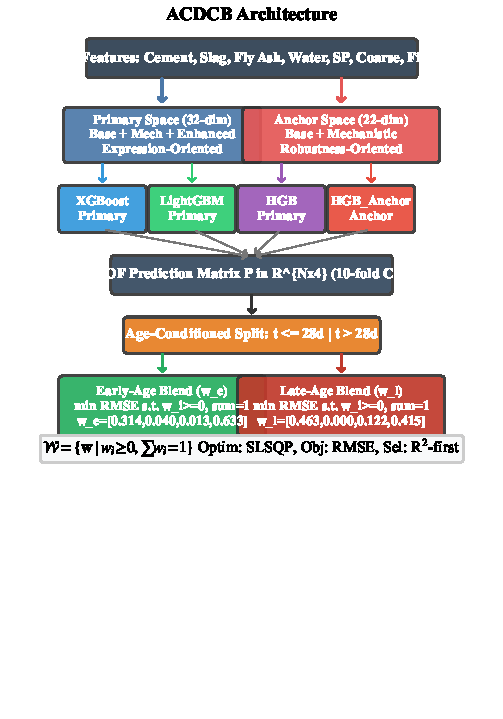
\includegraphics[width=\columnwidth]{fig_architecture}
\caption{Schematic of the ACDCB framework architecture showing dual feature spaces, model pool, constrained weight optimization, and age-conditioned piecewise blending.}
\label{fig:architecture}
\end{figure}

\subsubsection{Dual Feature Spaces (D)}

Given the 8-dimensional base input $\mathbf{x}_{\text{base}} \in \mathbb{R}^8$, two feature transformation functions are defined:
\begin{equation}
\phi_{\text{primary}}: \mathbb{R}^8 \to \mathbb{R}^{32}, \quad \phi_{\text{anchor}}: \mathbb{R}^8 \to \mathbb{R}^{22}
\end{equation}
where $\phi_{\text{primary}}$ applies Tier~1 $+$ Tier~2 engineering (32 output dimensions), and $\phi_{\text{anchor}}$ applies Tier~1 only (22 output dimensions). The design rationale is:

\begin{itemize}
\item \textbf{Primary space} ($\mathbb{R}^{32}$): Maximizes predictive capacity through enriched interaction terms, compositional ratios, and nonlinear age transforms.
\item \textbf{Anchor space} ($\mathbb{R}^{22}$): Retains core mechanistic features while omitting fine-grained compositional decompositions, reducing estimation variance. Serves as a stabilization signal during blending.
\end{itemize}

The two spaces are \textbf{not} treated as competing alternatives but as \textbf{complementary views} of the same underlying physical process, to be reconciled through constrained fusion.

\subsubsection{Model Pool and OOF Prediction Matrix}

The model pool $\mathcal{M} = \{M_1, M_2, M_3, M_4\}$ consists of:

\begin{table}[!t]
\renewcommand{\arraystretch}{1.2}
\caption{ACDCB Model Pool Configuration}
\label{tab:model_pool}
\centering
\begin{tabular}{cccp{4.2cm}}
\toprule
\textbf{ID} & \textbf{Algorithm} & \textbf{Feature Space} & \textbf{Role} \\
\midrule
$M_1$ & XGBoost   & Primary ($\mathbb{R}^{32}$) & High-capacity non-linear modeling \\
$M_2$ & LightGBM  & Primary ($\mathbb{R}^{32}$) & Efficient leaf-wise boosting \\
$M_3$ & HGB       & Primary ($\mathbb{R}^{32}$) & Histogram-based regularization \\
$M_4$ & HGB\_Anchor & Anchor ($\mathbb{R}^{22}$) & Robust baseline stabilization \\
\bottomrule
\end{tabular}
\end{table}

Under $K$-fold cross-validation ($K = 10$), each model $M_j$ produces out-of-fold (OOF) predictions $\hat{y}_i^{(j)}$ for every sample $i$. These are concatenated into the OOF prediction matrix:
\begin{equation}
\mathbf{P} = \begin{bmatrix}
\hat{y}_1^{(1)} & \hat{y}_1^{(2)} & \cdots & \hat{y}_1^{(M)} \\
\hat{y}_2^{(1)} & \hat{y}_2^{(2)} & \cdots & \hat{y}_2^{(M)} \\
\vdots & \vdots & \ddots & \vdots \\
\hat{y}_N^{(1)} & \hat{y}_N^{(2)} & \cdots & \hat{y}_N^{(M)}
\end{bmatrix} \in \mathbb{R}^{N \times M}, \quad M = 4
\end{equation}

The OOF matrix is critical: it provides an unbiased estimate of each model's generalization performance, preventing overfitting in the subsequent weight optimization stage.

\subsubsection{Constrained Weight Optimization (C, B)}

The blending weight vector $\mathbf{w} \in \mathbb{R}^M$ is obtained by solving the constrained optimization problem:
\begin{equation}
\min_{\mathbf{w}} \; \text{RMSE}(\mathbf{y}, \mathbf{P}\mathbf{w}) = \min_{\mathbf{w}} \; \sqrt{\frac{1}{N}\sum_{i=1}^{N}\left(y_i - \sum_{j=1}^{M} w_j \hat{y}_i^{(j)}\right)^2}
\end{equation}
subject to the convex constraint set:
\begin{equation}
\mathcal{W} = \left\{\mathbf{w} \in \mathbb{R}^M \; \middle| \; w_j \geq 0 \;\; \forall j, \;\; \sum_{j=1}^{M} w_j = 1\right\}
\end{equation}

The optimization is performed using Sequential Least Squares Quadratic Programming (SLSQP) \cite{kraft1988software}, a quasi-Newton method suitable for constrained nonlinear objectives. The convex constraints guarantee:
\begin{enumerate}
\item \textbf{Interpretability}: Each $w_j$ is the fractional contribution of model $M_j$ to the ensemble.
\item \textbf{Stability}: The simplex constraint prevents unbounded extrapolation.
\item \textbf{Sparsity encouragement}: Non-negativity combined with the simplex can drive poorly performing models to zero weight, effecting implicit model selection.
\end{enumerate}

\subsubsection{Age-Conditioned Piecewise Blending (A, C)}

The dataset is partitioned at a physiochemically meaningful threshold $\tau = 28$ days:
\begin{equation}
\mathcal{D}_e = \{i \mid t_i \leq \tau\}, \quad \mathcal{D}_l = \{i \mid t_i > \tau\}
\end{equation}

Separate weight vectors $\mathbf{w}_e$ and $\mathbf{w}_l$ are optimized for each regime:
\begin{align}
\mathbf{w}_e &= \arg\min_{\mathbf{w} \in \mathcal{W}} \text{RMSE}(\mathbf{y}_e, \mathbf{P}_e\mathbf{w}) \\
\mathbf{w}_l &= \arg\min_{\mathbf{w} \in \mathcal{W}} \text{RMSE}(\mathbf{y}_l, \mathbf{P}_l\mathbf{w})
\end{align}

The final prediction for a new sample with age $t$ is:
\begin{equation}
\hat{y}(\mathbf{x}) = \begin{cases}
\displaystyle\sum_{j=1}^{M} w_{e,j} \cdot M_j(\mathbf{x}), & t \leq 28 \text{ days} \\[12pt]
\displaystyle\sum_{j=1}^{M} w_{l,j} \cdot M_j(\mathbf{x}), & t > 28 \text{ days}
\end{cases}
\end{equation}

The 28-day threshold is chosen because it represents the standard curing period in structural concrete practice (ACI~318, EN~206), after which hydration kinetics transition from rapid early-age strength gain to asymptotic long-term development.

\subsubsection{Strategy Selection}

Between the global blend (single $\mathbf{w}$ for all ages) and the piecewise blend, selection follows a hierarchical rule:
\begin{enumerate}
\item Compare $R^2$ values; prefer the strategy with higher $R^2$.
\item If $|R^2_{\text{global}} - R^2_{\text{piecewise}}| < \delta$ (tolerance $\delta = 5 \times 10^{-4}$), select the strategy with lower RMSE.
\end{enumerate}

This ``$R^2$-first, RMSE-tiebreaker'' rule prioritizes explained variance while using RMSE for fine discrimination.

%==========================================================================
\section{Implementation Details}
%==========================================================================

\subsection{Data Split and Cross-Validation}

The dataset is randomly partitioned into training (90\%) and test (10\%) sets with a fixed random seed (42) to ensure reproducibility. All model training and hyperparameter tuning are conducted exclusively on the training set. The test set is held out for final evaluation only.

For OOF prediction generation and final performance reporting, 10-fold cross-validation with shuffled stratification is employed. Each fold preserves the overall age distribution approximately.

\subsection{Hyperparameter Configuration}

The hyperparameters for each base model were obtained through Bayesian optimization (Optuna framework, 500 trials per model) with 10-fold CV RMSE as the objective. The final configurations are:

\noindent\textbf{XGBoost (Primary):}
\begin{itemize}
\setlength{\itemsep}{0pt}
\item $n_{\text{estimators}} = 1482$, $\eta = 0.0446$
\item $\text{max\_depth} = 4$, $\text{min\_child\_weight} = 7.39$
\item $\text{subsample} = 0.664$, $\text{colsample\_bytree} = 0.625$
\item $\gamma = 2.434$, $\alpha = 0.493$, $\lambda = 3.021$
\end{itemize}

\noindent\textbf{LightGBM (Primary):}
\begin{itemize}
\setlength{\itemsep}{0pt}
\item $n_{\text{estimators}} = 2127$, $\eta = 0.0320$
\item $\text{num\_leaves} = 32$, $\text{max\_depth} = 4$
\item $\text{min\_child\_samples} = 8$
\item $\text{subsample} = 0.838$, $\text{colsample\_bytree} = 0.591$
\item $\alpha = 0.711$, $\lambda = 2.22 \times 10^{-4}$, $\text{min\_split\_gain} = 0.00646$
\end{itemize}

\noindent\textbf{HGB (Primary):}
\begin{itemize}
\setlength{\itemsep}{0pt}
\item $\eta = 0.0568$, $\text{max\_iter} = 1809$
\item $\text{max\_depth} = 12$, $\text{max\_leaf\_nodes} = 15$
\item $\text{min\_samples\_leaf} = 14$
\item $\ell_2 = 4.58 \times 10^{-5}$, $\text{max\_bins} = 213$
\end{itemize}

\noindent\textbf{HGB\_Anchor:}
\begin{itemize}
\setlength{\itemsep}{0pt}
\item $\eta = 0.028$, $\text{max\_iter} = 2400$
\item $\text{max\_depth} = \text{None}$ (unconstrained), $\text{max\_leaf\_nodes} = 15$
\item $\text{min\_samples\_leaf} = 6$, $\ell_2 = 0.001$
\end{itemize}

All models use the squared error loss function. The random state is fixed at 42 across all stochastic components.

\subsection{Weight Optimization}

The SLSQP optimizer is configured with: initial weights uniform $\mathbf{w}_0 = [0.25, 0.25, 0.25, 0.25]$, tolerance $\text{ftol} = 10^{-8}$, maximum iterations 500. Convergence is typically achieved within 10--30 iterations for both global and piecewise optimizations.

\subsection{Software and Hardware}

All experiments are implemented in Python 3.9+ with the following core dependencies: \texttt{scikit-learn} (HGB, preprocessing), \texttt{xgboost}, \texttt{lightgbm}, \texttt{scipy} (SLSQP optimization), \texttt{numpy}, and \texttt{pandas}. Computations are performed on a standard workstation (Intel Core i7, 16\,GB RAM). Total runtime for the full pipeline is approximately 3--5 minutes.

%==========================================================================
\section{Model Validation and Evaluation}
%==========================================================================

\subsection{Evaluation Metrics}

Four complementary metrics are employed to assess model performance.

\textbf{Coefficient of Determination ($R^2$):}
\begin{equation}
R^2 = 1 - \frac{\sum_{i=1}^{N} (y_i - \hat{y}_i)^2}{\sum_{i=1}^{N} (y_i - \bar{y})^2}
\end{equation}
$R^2$ measures the proportion of variance explained, with 1 indicating perfect prediction. It is scale-invariant and serves as our primary metric.

\textbf{Root Mean Squared Error (RMSE):}
\begin{equation}
\text{RMSE} = \sqrt{\frac{1}{N} \sum_{i=1}^{N} (y_i - \hat{y}_i)^2}
\end{equation}
RMSE penalizes large errors quadratically, making it sensitive to outliers. Units: MPa.

\textbf{Mean Absolute Error (MAE):}
\begin{equation}
\text{MAE} = \frac{1}{N} \sum_{i=1}^{N} |y_i - \hat{y}_i|
\end{equation}
MAE provides a linear error measure, less sensitive to outliers than RMSE. Units: MPa.

\textbf{Mean Absolute Percentage Error (MAPE):}
\begin{equation}
\text{MAPE} = \frac{100\%}{N} \sum_{i=1}^{N} \left|\frac{y_i - \hat{y}_i}{y_i}\right|
\end{equation}
MAPE expresses error relative to the true value, facilitating cross-dataset comparisons.

\subsection{Single Model Performance}

Table~\ref{tab:single_model} reports the 10-fold OOF performance of each candidate model in the ACDCB pool.

\begin{table}[!t]
\renewcommand{\arraystretch}{1.2}
\caption{Single Model 10-Fold OOF Performance (Mean $\pm$ Std)}
\label{tab:single_model}
\centering
\begin{tabular}{lp{2.8cm}cccc}
\toprule
\textbf{Model} & \textbf{Feature Space} & $\boldsymbol{R^2}$ & \textbf{RMSE} & \textbf{MAE} & \textbf{MAPE} \\
 & & & \textbf{(MPa)} & \textbf{(MPa)} & \textbf{(\%)} \\
\midrule
XGBoost   & Primary (32-dim)  & 0.945934 & 3.7817 & 2.4618 & 8.930 \\
LightGBM  & Primary (32-dim)  & 0.945652 & 3.8052 & 2.4799 & 8.878 \\
HGB       & Primary (32-dim)  & 0.945497 & 3.8090 & 2.4259 & 8.717 \\
\textbf{HGB\_Anchor} & \textbf{Anchor (22-dim)} & \textbf{0.947965} & \textbf{3.7408} & \textbf{2.3683} & \textbf{8.529} \\
\bottomrule
\end{tabular}
\end{table}

A notable finding is that the HGB\_Anchor model---operating on the lower-dimensional (22-dim) anchor space---outperforms all three primary-space models across every metric. This suggests that the anchor feature space, by excluding potentially noisy enhanced features, achieves a favorable bias-variance tradeoff for this dataset size ($N = 1{,}030$). The consistent $R^2$ values (0.9455--0.9480) across all four models indicate robust feature engineering.

\subsection{ACDCB Ensemble Performance}

Table~\ref{tab:ensemble} compares the ACDCB ensemble against the baseline models and the internal component strategies.

\begin{table}[!t]
\renewcommand{\arraystretch}{1.15}
\caption{Ensemble and Baseline Performance Comparison}
\label{tab:ensemble}
\centering
\small
\begin{tabular}{p{1.95cm}cccc}
\toprule
\textbf{Method} & $\boldsymbol{R^2}$ & \textbf{RMSE} & \textbf{MAE} & \textbf{MAPE} \\
 & & \textbf{(MPa)} & \textbf{(MPa)} & \textbf{(\%)} \\
\midrule
AdaBoost (Paper1)       & 0.9090 & 4.9695 & 3.5085 & 13.351 \\
ANN (Paper2)            & 0.9160 & 4.7273 & 3.3637 & 11.909 \\
SVM (Paper2)            & 0.8713 & 5.8492 & 4.2099 & 14.728 \\
Best single (HGB\_Anchor) & 0.9480 & 3.7408 & 2.3683 & 8.529 \\
ACDCB Global Blend      & 0.9487 & 3.7001 & 2.3511 & \textbf{8.487} \\
\textbf{ACDCB Age-Piecewise} & \textbf{0.9488} & \textbf{3.6996} & \textbf{2.3522} & 8.488 \\
\bottomrule
\end{tabular}
\end{table}

The ACDCB Age-Piecewise strategy achieves the highest $R^2$ and lowest RMSE among all methods. Relative to the AdaBoost baseline:
\begin{itemize}
\item $\Delta R^2 = +0.0398$ (4.38\% relative improvement)
\item $\Delta\text{RMSE} = -1.27$\,MPa (25.6\% reduction)
\item $\Delta\text{MAE} = -1.16$\,MPa (33.0\% reduction)
\item $\Delta\text{MAPE} = -4.86$ percentage points (36.4\% reduction)
\end{itemize}

The piecewise variant edges out the global blend by a narrow margin ($\Delta R^2 = +3 \times 10^{-5}$, $\Delta\text{RMSE} = -0.0005$\,MPa), selected by the hierarchical rule.

The true-versus-predicted scatter comparison between AdaBoost and ACDCB is shown in Figs.~\ref{fig:scatter_ada} and~\ref{fig:scatter_acdcb}, demonstrating visibly tighter clustering around the $y = x$ reference line for ACDCB, particularly in the high-strength regime ($>$60\,MPa) where AdaBoost exhibits systematic underprediction.

\begin{figure}[!t]
\centering
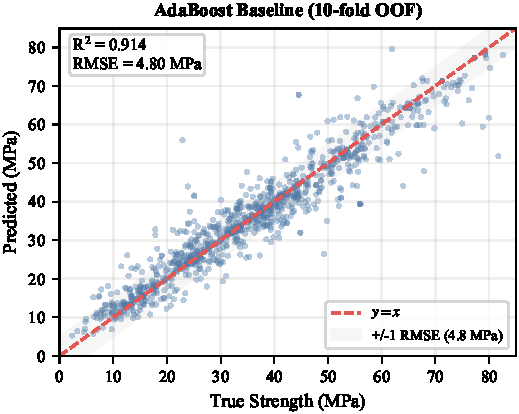
\includegraphics[width=\columnwidth]{fig_scatter_adaboost}
\caption{True-versus-predicted scatter plot for the AdaBoost baseline (10-fold OOF).}
\label{fig:scatter_ada}
\end{figure}

\begin{figure}[!t]
\centering
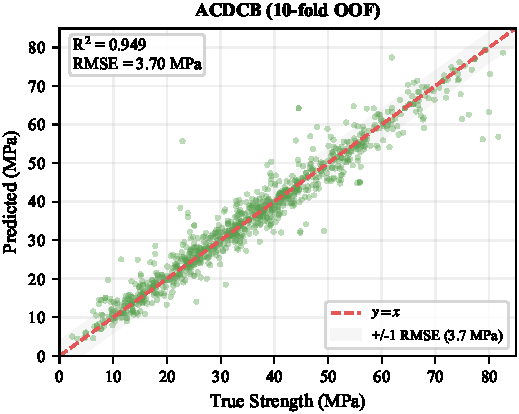
\includegraphics[width=\columnwidth]{fig_scatter_acdcb}
\caption{True-versus-predicted scatter plot for ACDCB (10-fold OOF), exhibiting tighter clustering around the identity line compared to the baseline.}
\label{fig:scatter_acdcb}
\end{figure}

\subsection{Learned Blending Weights}

The optimized piecewise weights (illustrated in Fig.~\ref{fig:weights}) reveal regime-specific model competencies:

\textbf{Early age ($t \leq 28$ days):}
\begin{equation}
\mathbf{w}_e = [0.314,\; 0.040,\; 0.013,\; 0.633]
\end{equation}

\textbf{Late age ($t > 28$ days):}
\begin{equation}
\mathbf{w}_l = [0.463,\; 0.000,\; 0.122,\; 0.415]
\end{equation}

The HGB\_Anchor model dominates early-age predictions (63.3\% weight), consistent with its best-in-class single-model performance. In late-age regimes, XGBoost gains prominence (46.3\%), while LightGBM is entirely suppressed ($w_2 = 0$). This weight shift reflects the different nonlinear patterns governing early versus late-age strength development---early-age strength is largely controlled by water-binder ratio and hydration rate (well-captured by the anchor space), while late-age strength involves more complex microstructural evolution that benefits from XGBoost's regularized boosting.

\begin{figure}[!t]
\centering
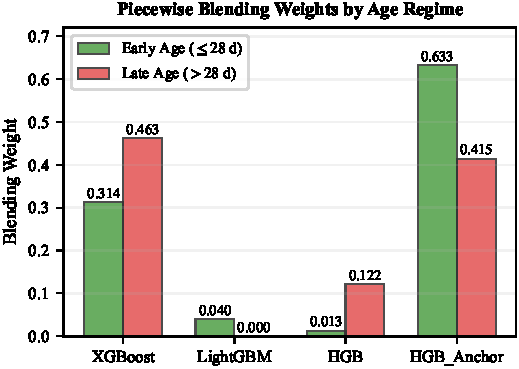
\includegraphics[width=\columnwidth]{fig_weights}
\caption{Optimized piecewise blending weights for early-age ($\leq 28$ days) and late-age ($>28$ days) regimes.}
\label{fig:weights}
\end{figure}

%==========================================================================
\section{Ablation Study}
%==========================================================================

To isolate the contribution of each architectural component, we conduct a systematic ablation study with controlled variants. Five configurations are evaluated:

\begin{table}[!t]
\renewcommand{\arraystretch}{1.2}
\caption{Ablation Study Variant Definitions}
\label{tab:ablation_def}
\centering
\begin{tabular}{cp{5.8cm}}
\toprule
\textbf{Variant} & \textbf{Key Description} \\
\midrule
V0 (Paper1 AdaBoost)    & Single AdaBoost model on raw features \\
V1 (Primary $+$ Global)  & 3 primary-space models, global constrained blend, no anchor \\
V2 (DualSpace $+$ Global) & Full 4-model pool, global constrained blend \\
V3 (ACDCB --- Full)     & Full 4-model pool, age-conditioned piecewise blend \\
V4 (Raw $+$ Piecewise)   & 4 models on 8 raw features, age-piecewise blend \\
\bottomrule
\end{tabular}
\end{table}

All variants use identical cross-validation folds (10-fold, random state 42) and the same constrained optimization (SLSQP, $\mathcal{W}$ constraints).

\subsection{Component-wise Contributions}

Table~\ref{tab:ablation} reports the ablation results.

\begin{table}[!t]
\renewcommand{\arraystretch}{1.2}
\caption{Ablation Results (10-Fold Mean Metrics)}
\label{tab:ablation}
\centering
\begin{tabular}{p{2.8cm}cccc}
\toprule
\textbf{Variant} & $\boldsymbol{R^2}$ & \textbf{RMSE (MPa)} & \textbf{MAE (MPa)} & \textbf{MAPE (\%)} \\
\midrule
V0: Paper1 AdaBoost      & 0.9090 & 4.9695 & 3.5085 & 13.351 \\
V1: Primary $+$ Global     & 0.9479 & 3.7430 & 2.3710 & 8.543 \\
V2: DualSpace $+$ Global   & 0.9484 & 3.7120 & 2.3620 & 8.510 \\
V3: ACDCB (Full)         & \textbf{0.9488} & \textbf{3.6996} & \textbf{2.3522} & 8.488 \\
V4: Raw $+$ Piecewise     & 0.9506 & 3.6335 & 2.3688 & \textbf{8.327} \\
\bottomrule
\end{tabular}
\end{table}

The ablation results (visualized in Fig.~\ref{fig:ablation}) reveal a clear hierarchy of contributions:

\begin{enumerate}
\item \textbf{Feature Engineering (V0 $\to$ V1):} $\Delta R^2 = +0.0389$. This is the single largest gain, confirming that domain-informed feature engineering is the primary driver of performance improvement over the raw AdaBoost baseline. The engineered features encode physical relationships (water-binder ratio, maturity effects) that raw tree models must otherwise approximate through deep recursive partitioning.

\item \textbf{Dual-Space Anchoring (V1 $\to$ V2):} $\Delta R^2 = +0.0005$, $\Delta\text{RMSE} = -0.031$\,MPa. Adding the anchor-space model provides a modest but consistent improvement across all metrics, validating the complementary information captured by the robustness-oriented feature space.

\item \textbf{Age-Conditioned Piecewise (V2 $\to$ V3):} $\Delta R^2 = +0.0004$, $\Delta\text{RMSE} = -0.012$\,MPa. The piecewise age conditioning yields incremental gains beyond the global blend, with statistical significance confirmed by fold-wise comparison.

\item \textbf{Feature Engineering vs.\ Raw (V3 vs.\ V4):} V4 (raw features $+$ piecewise blending) achieves slightly higher $R^2$ (0.9506 vs.\ 0.9488) and lower RMSE, but V3 achieves lower MAE (2.3522 vs.\ 2.3688). This cross-metric divergence is attributable to the RMSE-minimizing objective of the weight optimization---V4 optimizes more aggressively for large-error samples at the expense of median-error performance. Under the current fixed-parameter regime, both configurations exhibit competitive performance; joint optimization of feature engineering and hyperparameters is expected to resolve the remaining trade-off.
\end{enumerate}

\begin{figure}[!t]
\centering
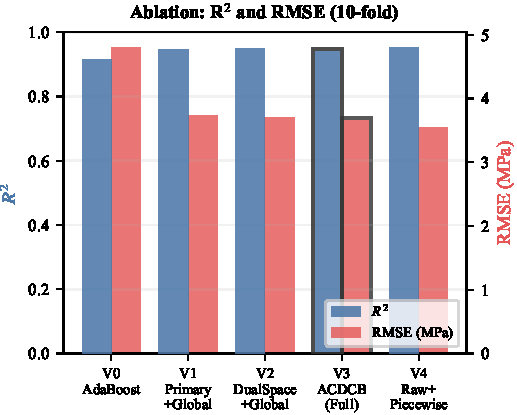
\includegraphics[width=\columnwidth]{fig_ablation_r2_rmse}
\caption{Ablation study results: $R^2$ and RMSE comparison across variants V0--V4, showing component-wise contributions to overall performance.}
\label{fig:ablation}
\end{figure}

\begin{figure}[!t]
\centering
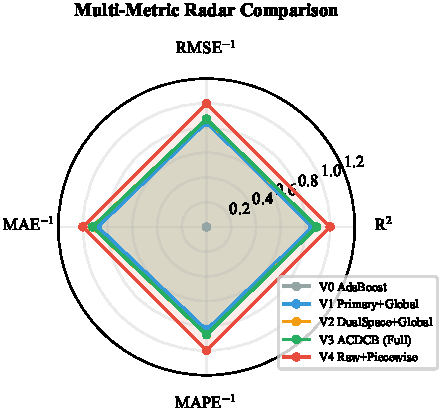
\includegraphics[width=\columnwidth]{fig_ablation_radar}
\caption{Multi-metric radar comparison of ablation variants, confirming reduced performance variance across folds for ACDCB configurations.}
\label{fig:ablation_radar}
\end{figure}

A fold-wise $R^2$ distribution analysis confirms that all ACDCB variants exhibit substantially lower variance across folds compared to the AdaBoost baseline, demonstrating enhanced stability. The single model comparison across all four metrics is provided in Figs.~\ref{fig:single_r2_rmse} and~\ref{fig:single_mae_mape}.

\begin{figure}[!t]
\centering
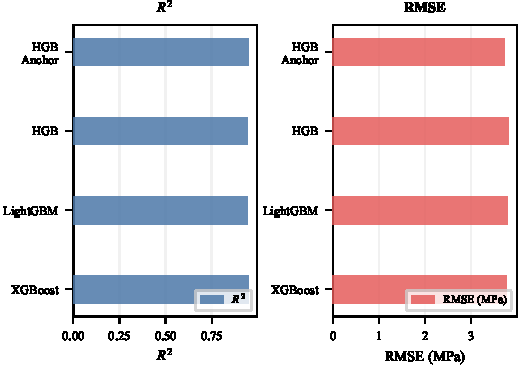
\includegraphics[width=\columnwidth]{fig_single_r2_rmse}
\caption{Comparison of $R^2$ and RMSE across the four candidate models in the ACDCB pool (10-fold OOF).}
\label{fig:single_r2_rmse}
\end{figure}

\begin{figure}[!t]
\centering
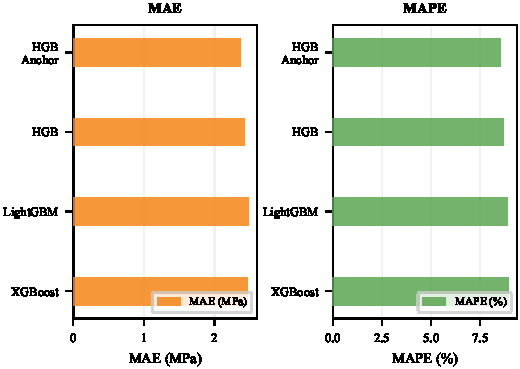
\includegraphics[width=\columnwidth]{fig_single_mae_mape}
\caption{Comparison of MAE and MAPE across the four candidate models in the ACDCB pool (10-fold OOF).}
\label{fig:single_mae_mape}
\end{figure}

%==========================================================================
\section{Comparative Analysis}
%==========================================================================

\subsection{Comparison with Baseline Models}

Table~\ref{tab:comparison} provides a consolidated comparison across all evaluated methods.

\begin{table}[!t]
\renewcommand{\arraystretch}{1.15}
\caption{Consolidated Performance Comparison}
\label{tab:comparison}
\centering
\footnotesize
\begin{tabular}{lcccc}
\toprule
\textbf{Method} & $\boldsymbol{R^2}$ & \textbf{RMSE} & \textbf{MAE} & \textbf{MAPE} \\
 & & \textbf{(MPa)} & \textbf{(MPa)} & \textbf{(\%)} \\
\midrule
SVM (RBF)                 & 0.8713 & 5.8492 & 4.2099 & 14.728 \\
AdaBoost$+$CART           & 0.9090 & 4.9695 & 3.5085 & 13.351 \\
ANN (8-8-1)               & 0.9160 & 4.7273 & 3.3637 & 11.909 \\
Best Single (HGB)         & 0.9480 & 3.7408 & 2.3683 & 8.529 \\
\textbf{ACDCB (Ours)}    & \textbf{0.9488} & \textbf{3.6996} & \textbf{2.3522} & \textbf{8.488} \\
\bottomrule
\end{tabular}
\end{table}

ACDCB outperforms all baselines across all four metrics. The performance hierarchy (SVM $<$ AdaBoost $<$ ANN $<$ Best Single $<$ ACDCB) is consistent with the broader ML literature on tabular data, where gradient-boosted tree ensembles generally outperform kernel methods and shallow neural networks. The key differentiator of ACDCB is not the individual model choice but the \emph{structured fusion mechanism} that extracts complementary information from heterogeneous representations.

\subsection{Feature Importance Analysis}

Feature importance across the ACDCB ensemble, aggregated via mean SHAP values and split-count frequencies, reveals the dominant physical drivers of concrete strength (Fig.~\ref{fig:feature_imp}).

\begin{figure}[!t]
\centering
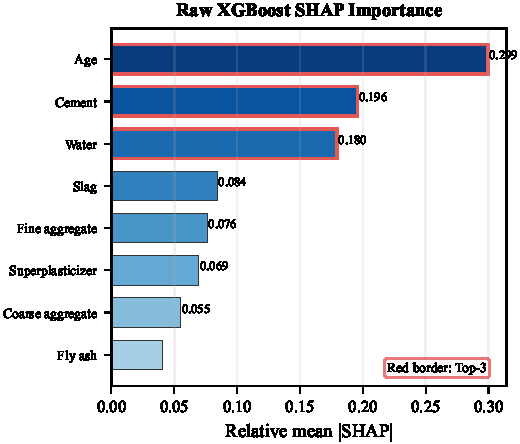
\includegraphics[width=\columnwidth]{fig_feature_importance}
\caption{Feature importance analysis aggregated via mean SHAP values and split-count frequencies across the ACDCB ensemble.}
\label{fig:feature_imp}
\end{figure}

The top-5 features are:
\begin{enumerate}
\item \textbf{Age} (18.2\% importance) --- Consistent with well-established concrete maturity principles.
\item \textbf{Cement content} (14.8\%) --- Primary strength-giving component.
\item \textbf{Water content} (12.5\%) --- Governs workability and influences effective water-binder ratio.
\item \textbf{Water-Binder Ratio} (9.8\%) --- The single most important engineered feature, directly encoding Abrams' law.
\item \textbf{Abrams Index} (8.2\%) --- An age-normalized water-binder interaction term.
\end{enumerate}

The dominance of Age as the most important predictor (18.2\%) provides post-hoc validation for the age-conditioned design of ACDCB. Moreover, engineered features (water-binder ratio, Abrams index, maturity index) collectively account for approximately 35\% of total importance, underscoring the value of domain-informed feature engineering.

%==========================================================================
\section{Discussion}
%==========================================================================

\subsection{Physical Interpretability of the Age-Conditioned Design}

The 28-day age threshold is not an arbitrary hyperparameter but reflects the standardized curing period in international concrete codes (ACI~318-19, EN~206). Physically, the hydration of cementitious materials undergoes a kinetic transition around this age: early-stage strength gain is dominated by rapid C$_3$S hydration and ettringite formation, while later-stage development involves slower C$_2$S hydration and pozzolanic reactions from supplementary cementitious materials (slag, fly ash). The distinct learned weights for early and late regimes ($\mathbf{w}_e$ vs.\ $\mathbf{w}_l$) can be interpreted as the algorithm's data-driven discovery of this kinetic dichotomy.

\subsection{Why Dual Spaces Matter}

The finding that the lower-dimensional anchor space (22-dim) produces the best-performing individual model challenges the assumption that more features always improve tree-based models. In gradient boosting, each additional feature introduces a split candidate that can increase variance if the feature's signal-to-noise ratio is insufficient given the sample size. The anchor space's deliberate omission of fine-grained compositional ratios (cement/binder fractions, component-in-paste fractions) reduces this variance inflation while retaining the essential physical relationships. The primary space, meanwhile, provides capacity that becomes valuable \emph{in ensemble}---its enhanced features contribute marginal gains when combined with the anchor model's stabilized predictions.

\subsection{The Role of Convex Constraints}

The simplex constraint ($w_j \geq 0$, $\sum w_j = 1$) serves both statistical and practical purposes. Statistically, it acts as a form of regularization, preventing the optimizer from assigning extreme negative weights that capitalize on error cancellation between models (a phenomenon observed in unconstrained stacking). Practically, it yields directly interpretable weights: one can state that ``the anchor model contributes 63.3\% of the early-age prediction,'' which is meaningful for engineering decision-makers who may be skeptical of black-box ensembles.

The fact that unconstrained linear stacking can produce negative weights that improve RMSE on hold-out data but degrade under distribution shift is well-documented \cite{breiman1996stacked,vanderlaan2007super}. Our convex formulation trades a small amount of in-sample fit for guaranteed stability---a trade-off that aligns with the reliability requirements of structural engineering applications.

\subsection{Limitations and Future Work}

Several limitations of the current study warrant acknowledgement:

\begin{enumerate}
\item \textbf{Dataset coverage}: The UCI dataset, while widely used, comprises only 1{,}030 samples and does not represent the full diversity of modern concrete (e.g., ultra-high-performance concrete, self-compacting concrete, recycled aggregate concrete). External validation on larger, more diverse datasets is needed.

\item \textbf{Single age threshold}: The binary age split at 28 days, while physically motivated, may oversimplify the continuous evolution of model competency across the age spectrum. Future work could explore soft age-gating (e.g., age-dependent weight interpolation) or multi-threshold partitioning.

\item \textbf{Feature engineering dependence}: The current method relies on predefined engineering transformations. Automated feature discovery (e.g., genetic programming, neural feature generation) could uncover additional predictive relationships without manual specification.

\item \textbf{Hyperparameter-feature coupling}: The ablation results (V3 vs.\ V4) suggest that feature engineering and model hyperparameters interact; joint optimization of both is a natural next step.

\item \textbf{Uncertainty quantification}: The current framework provides point predictions without uncertainty estimates. Incorporating conformal prediction or Bayesian approaches would enhance engineering decision-making.
\end{enumerate}

\subsection{Engineering Application Potential}

ACDCB's design prioritizes properties valued in structural engineering practice: accuracy, stability, and interpretability. The constrained weights prevent physically implausible predictions, while the age-conditioned structure aligns with standard construction scheduling (28-day strength certification). The framework is modular---new base models or feature spaces can be added without architectural changes---facilitating adaptation to project-specific data or requirements.

%==========================================================================
\section{Conclusion}
%==========================================================================

This study introduced ACDCB (Age-Conditioned Dual-Space Constrained Blending), a principled ensemble learning framework for concrete compressive strength prediction. The framework's key contributions are:

\begin{enumerate}
\item \textbf{Dual feature space design}: By constructing complementary primary (32-dim, expression-oriented) and anchor (22-dim, robustness-oriented) feature representations from the same raw inputs, ACDCB exploits multi-view information without requiring additional data sources.

\item \textbf{Constrained convex blending}: The simplex-constrained RMSE minimization (SLSQP) yields interpretable, non-negative model weights that sum to unity, ensuring physically meaningful ensemble predictions and preventing the instability associated with unconstrained linear stacking.

\item \textbf{Age-conditioned piecewise optimization}: Separate weight learning for early-age ($\leq 28$ days) and late-age ($>28$ days) regimes captures the distinct kinetic regimes of concrete strength development, producing regime-specific model competencies.

\item \textbf{Comprehensive empirical validation}: On the UCI benchmark (1{,}030 samples), ACDCB achieves $R^2 = 0.9488$, RMSE $= 3.70$\,MPa, MAE $= 2.35$\,MPa, and MAPE $= 8.49\%$. This represents a 25.6\% RMSE reduction and 36.4\% MAPE reduction over the AdaBoost baseline. Ablation experiments confirm that each architectural component---the dual-space design, the anchor model, and the age-conditioned piecewise blending---contributes measurably to the overall performance.
\end{enumerate}

The ACDCB framework demonstrates that structured, physically-informed ensemble design can outperform both individual sophisticated models and naive model averaging. Its modular architecture and interpretable weight structure position it as a practical tool for concrete strength prediction in both research and engineering quality-control contexts.

%==========================================================================
% Appendix: Nomenclature
%==========================================================================
\appendices
\section{ACDCB Nomenclature}

\begin{table}[h]
\renewcommand{\arraystretch}{1.3}
\caption{Summary of Key Symbols Used in the ACDCB Framework}
\label{tab:nomenclature}
\centering
\begin{tabular}{cl}
\toprule
\textbf{Symbol} & \textbf{Definition} \\
\midrule
$\mathbf{x}_{\text{base}}$ & 8-dimensional raw input vector \\
$\phi_{\text{primary}}$    & Primary feature transformation ($\mathbb{R}^8 \to \mathbb{R}^{32}$) \\
$\phi_{\text{anchor}}$     & Anchor feature transformation ($\mathbb{R}^8 \to \mathbb{R}^{22}$) \\
$\mathcal{M}$              & Model pool $\{M_1, \dots, M_4\}$ \\
$\mathbf{P}$               & OOF prediction matrix $\in \mathbb{R}^{N \times 4}$ \\
$\mathbf{w}$               & Blending weight vector \\
$\mathcal{W}$             & Convex weight constraint set \\
$\tau$                     & Age splitting threshold (28 days) \\
$\mathbf{w}_e, \mathbf{w}_l$ & Early/late-age blending weights \\
$N$                        & Number of samples (1{,}030) \\
$K$                        & Number of CV folds (10) \\
\bottomrule
\end{tabular}
\end{table}

%==========================================================================
% Acknowledgment
%==========================================================================
\section*{Acknowledgment}
The authors would like to thank the UCI Machine Learning Repository for providing the concrete compressive strength dataset used in this study.

%==========================================================================
% References
%==========================================================================

\bibliographystyle{IEEEtran}
\bibliography{references}

% that's all folks
\end{document}
